%% This file is a portion of the source for Revised Edition 1.1 of
%% Operating Systems and Middleware: Supporting Controlled
%% Interaction, Copyright 2011 by Max Hailperin.  This work is
%% licensed under the Creative Commons Attribution-ShareAlike 3.0
%% Unported License. To view a copy of this license, visit
%% http://creativecommons.org/licenses/by-sa/3.0/ or send a letter to
%% Creative Commons, 171 Second Street, Suite 300, San Francisco,
%% California, 94105, USA.
\chapter{Stacks}\label{stacks-appendix}

Most compilers for higher-level programming languages produce
machine-language object code that makes crucial use of a stack stored
in the computer's memory.  This stack is used to allocate space
whenever a procedure is called and then deallocate the space when the
procedure returns.  That is, the space is associated with a particular
activation of a procedure, and as such, is called an \vocab{activation
record}.  For this reason, the stack is called an
\foldvocab{activation record}{stack}.  Another name for the same stack
is the \foldvocab{runtime}{stack}, because it plays a central role in
the \vocab{runtime environment}, which is to say, the supporting
structures the compiler expects to be present at the time the object
code is run.  Even programs written in assembly language generally
make use of an activation record stack, because assembly programmers
normally write their procedures following the same conventions as are
used by compilers.

You may have studied activation record stacks in a course on
programming languages, compilers, or computer organization; you may
even have learned something about them in an introductory computer
science course.  If you have not previously studied this topic, this appendix should suffice.  For the
purposes of understanding operating systems, you do not need to know
all the details of how activation records are used.  However, you do
need some understanding of how the stack space is allocated in order
to understand Chapter~\ref{threads-chapter}'s explanation of thread
switching and also as background for one of the security issues
discussed in Chapter~\ref{security-chapter}.  Therefore, in
Section~\ref{stacks-abstract-section}, I provide an overview of what
stack-allocated storage is, and in Section~\ref{stacks-concrete-section}, I
explain how this storage is represented using memory and a register.
Then, in Section~\ref{stacks-application-section}, I sketch how this is
used to support procedure activations.

\section{Stack-Allocated Storage: The Concept}\label{stacks-abstract-section}

Like most authors writing about computer systems, I use the word
\vocab{stack} to refer to stack-allocated storage, which is a
generalization of the simpler variety of stack used in the
mathematical study of algorithms.  I will first describe the
simpler kind of stack, and then I will explain how stack-allocated storage goes
beyond it.

The simple kind of stack is a modifiable object supporting two
operations: \vocab{push} and \vocab{pop}.  Each of these operations
modifies the stack's state, which can be thought of as a sequence of
values arranged in chronological order according to when they were added to
the stack.  When a new stack is created, it does not hold any values.
The push operation adds one new value as the most recent one.  The pop
operation removes the most recent value and returns it.  Because the
pop operation changes the stack's state, the next pop will generally
produce a different result.  You can think of pop as returning the
most recently pushed value that has not yet been popped.  This value
is said to be at the top of the stack.  Note that it is illegal to pop from an
empty stack.

As an example of how this simple kind of stack operates, suppose a new stack is created, and then
the values 3 and 1 are pushed on it, in that order.  If a pop
operation is done, the top element, 1, is returned.  After this pop
operation, the 1 is no longer on the stack, and so a second pop would
return the 3 that is now on top.  A third pop would be illegal, because the
first two pops leave the stack empty.

Stack-allocated storage provides a collection of memory locations that
can be individually loaded from or stored into, much like the elements
of an array.  However, the collection of locations can expand and
contract in a stack-like fashion.

I can now explain the operations available on a stack, in the sense of
a stack-allocated storage structure.  Each newly created stack starts
with a size of zero.  That is, while the underlying representation may
already be occupying memory space, there are no memory locations valid
for loading and storing.  The stack at this point is much like a
zero-length array.

The size of the stack can be expanded using an allocate operation,
which takes a parameter specifying how many new memory locations
should be made available.  The newly allocated memory locations are
guaranteed to be located at consecutive addresses, and the allocate
operation returns the smallest of these addresses.  Thus, each
location within the allocated block of storage can be loaded or stored
using an address calculated as some offset from the base address
returned by the allocation.

The size of the stack can be decreased using a deallocate operation,
again with a parameter specifying the number of locations to be
removed.  Because the storage is managed in a stack-like fashion, a
deallocate operation frees up the most recently allocated storage
locations that have not already been deallocated.  Once storage
locations are deallocated, it is illegal to use their addresses for
loading or storing.

Normally the size of each deallocation request matches the size of a
corresponding allocation request.  For example, one might allocate 16
locations,  allocate 48 more,  deallocate the top 48, and
finally deallocate the remaining 16.  A single deallocation request can
also combine the sizes from several allocations.  For instance, all 64
locations in the preceding example could be deallocated at once.  The only
complicated kind of deallocation request is one that frees up some, but not
all, of a block of memory locations that were allocated together.  In
that case, the stack implementation needs to specify which locations
in the partially deallocated block remain valid.  I will not pursue
this issue further, as it isn't relevant to the matters at hand.
Instead, I will turn to the realities of how stacks are represented
within computer hardware.

\section{Representing a Stack in Memory}\label{stacks-concrete-section}

The standard representation of a stack is a large region of
consecutive memory locations together with a \vocab{stack pointer}
register that indicates how many of the locations are in use.  The
size of the region is chosen to be large enough that the stack normally
will not overflow it.  The virtual memory system (described in
Chapter~\ref{vm-chapter}) can enforce this limit and can also expand
the size of the region if necessary, provided the adjoining addresses
are not in use for another purpose.

The allocated locations within the stack are all at one end of the
region of memory.  One possibility is that the allocated locations
occupy the lowest addresses in the region and that each allocation request
expands the stack upward into the higher addresses.  The other
possibility is that the allocated locations occupy the highest
addresses in the region and that allocation requests expand the stack
downward into lower addresses.  The latter arrangement is the more
common in practice, and so I will assume it for the remainder of my
explanation.

The stack pointer register indicates how much of the memory region is
in use.  It does this not by containing a count of how many locations
are currently allocated, but by holding the address of the most
recently allocated location.  This location is conceptually the
``top'' of the stack, though because the stack grows downward, the
word ``top'' is misleading.  The stack pointer contains the
numerically smallest memory address of any currently allocated
location.  Figure~\ref{example-stack} shows a stack after allocating 16
locations and then 48; the stack pointer contains the 64th largest
memory address in the region. (In some architectures, the stack pointer
points to the free memory location that would be the next one allocated,
rather than to the most recently allocated location.  This would move the pointer one location lower, but does not make any significant difference
for the purposes of this book.)
\begin{figure}
\centerline{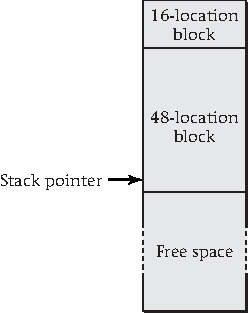
\includegraphics{hail_f0a01}}
%\centerline{\def\epsfsize#1#2{0.6#1}\epsfbox{example-stack.eps}}
\caption{A stack grows downward, occupying the highest addresses in
  the region used to store it.  The stack pointer points at the
  ``top'' of the stack, that is, the most recently allocated block of
  space.  In this example, blocks of size 16 and 48 were allocated, so
  the stack pointer points at the 64th location from the end of the
  memory region.}
\label{example-stack}
\end{figure}

Given this representation, an allocate operation decreases the stack
pointer by the number of locations requested and returns the new
stack pointer value as the base address of the allocated block.  A
deallocate operation increases the stack pointer by the number of
locations to be freed.  For example, deallocating 48 locations in
Figure~\ref{example-stack} would leave the stack pointer pointing at the
lowest-numbered address of the 16 locations in the remaining block of
storage.

At this point, you should understand the basic management of stack
space, but not the purpose to which that space is put.  Therefore, I
will provide a brief synopsis of how programming-language
implementations make use of stack space.

\section{Using a Stack for Procedure Activations}\label{stacks-application-section}

When one procedure calls another, the caller executes an instruction that
jumps to the beginning of the called procedure.  That instruction also
stores a \vocab{return address}, which is the address of the calling
procedure's next instruction after the procedure call.  That way,
when the called procedure is ready to return, it can jump to the
return address and thereby resume execution of the calling procedure.

Computer architectures differ in where they store the return address.
One approach is for the procedure call instruction to push the return
address on the stack.  This approach is used in the popular IA-32
architecture, which is also known as the x86 architecture, and is
implemented by processors such as those in the Pentium family.  Thus, the very
first element of a procedure activation record may be the return
address, pushed by the procedure call instruction itself.

In other architectures, such as MIPS, the procedure call
instruction places the return address in a register.  If the called
procedure does not execute any further procedure calls before it
returns, the return address can remain in the register.  The return
instruction jumps to the address stored in the register.  In this
case, where there are no further procedure calls, the procedure
activation is termed a \vocab{leaf}.

However, this register-based approach to return addresses does not
directly support nesting of procedure activations, with the called
procedure in turn calling a third procedure, which may call a fourth,
and so on.  To support that nesting, a whole chain of return addresses
is needed; the innermost procedure activation must be able to return
to its caller, which in turn must be able to return to its caller, and
so forth.  One register cannot hold all these return addresses
simultaneously.  Therefore, any nonleaf procedure activation must
store the return address register's value into the activation record
and later retrieve it from there.  As a result, the activation records
hold return addresses, even on architectures that don't directly push
the return address onto the stack in the first place.

Each procedure activation also needs some storage space for local
variables and other values that arise in the course of the procedure's
computation.  Some of this storage may be in registers rather than in
memory.  When one procedure calls another, there must be some
agreement regarding how they will share the registers.  Typically the
agreement specifies that the called procedure must leave some
registers the way it found them, that is, containing the same values
at procedure return as at procedure entry.  The calling procedure can
leave its values in these registers when it executes the procedure
call.  Other registers can be freely modified by the called procedure;
the calling procedure must not leave any important values in them.

Either kind of register is likely to be saved into the stack.  If the
called procedure promises to leave a register as it found it, but
wants to use that register for its own storage, it will reconcile this
conflict by saving the register to the stack before modifying it and then
restoring the saved value before returning.  Thus, the caller will
never know that the register was temporarily modified.  This
approach is known as \vocab{callee saves}, because the callee saves
the register
into its activation record.

For registers that the callee may overwrite without compunction, the
situation is somewhat different.  For these registers, it is the caller that may
want to save them into its own activation record.  The caller saves
the registers before the procedure
call and restores them upon resumption.  Therefore, this
approach is known as \vocab{caller saves}.

Each architecture has some convention for which registers are
preserved using the caller-saves approach and which using the
callee-saves approach.  That way,
any two procedures will correctly interoperate.  The details don't
matter for the purposes of this book; what matters is that activation
records hold saved registers.  As such, the stack is also a natural
place for saving registers upon thread switching, as described in 
Chapter~\ref{threads-chapter}.

Some values local to a procedure activation cannot be stored in
registers.  For example, suppose that a procedure makes use of a local
array, which is allocated when the procedure is entered and
deallocated when the procedure returns.  This array will be stored in
memory so that the array elements can be accessed with load and store
instructions.  Because the lifetime of the array corresponds with a
procedure activation, the array will be part of the activation
record.  In Chapter~\ref{security-chapter}, I explain that this can
create a security risk if input is read into the array without checking
the amount of input versus the array size.  As I explain there,
if the input runs past the end of the array, it can overwrite other
parts of the procedure's activation record, or the activation records
of the caller, the caller's caller, and so forth, with potentially
dangerous results.
